\chapter{Data \& Methods}
\label{ch:methods}

\blockquote{This chapter describes the data used for this study, and how those data were analyzed. It covers the selection criteria for languages and lexemes, which corpora were used, and how the data were obtained and formatted. I also describe the methods used to annotate the data, and factors that influenced how the data were coded. I present and explain a measure of corpus dispersion that is used partly in place of, and partly as a complement to, raw frequencies of lexemes. Lastly, I set forth a procedure for operationalizing and quantifying lexical flexibility in a crosslinguistically comparable way. The formulation of this lexical flexibility measure is a key methodological contribution of this thesis.}

\section{Introduction}
\label{sec:3.1}

The process of collecting, annotating, and analyzing the data for this study adheres to several self-imposed principles. First and foremost, the data in this study are naturalistic discourse data rather than elicited data. This principle has two motivations: First, as discussed in \secref*{sec:1.2}, few studies examine token frequencies of lexical items used for different discourse functions, and those that do only report aggregated results. Most extant research consists of lexicon-based counts. This study therefore explores a previously unexamined aspect of lexical flexibility. Second, corpus-based methods study real-world instances of language in use, rather than made-up examples or examples produced by introspection, which are subject to various cognitive and social biases \parencite[168]{Baker2018}. Corpus data are also more likely to reveal prototype effects through statistical tendencies. For this study, I relied on specialized corpora of spoken narrative and conversational texts only. This ensures greater comparability between the corpora used in this study and other documentary corpora that these methods may be applied to in the future, since most documentary corpora likewise consist of spoken narratives and conversations.

The second self-imposed requirement for this study is adherence to the \href{https://site.uit.no/linguisticsdatacitation/}{Austin principles of data citation in linguistics} \parencite{BerezKroekeretal2018}. In particular, the source for each data point discussed in this thesis is uniquely identified with its location in the corpus, and the data used in this study are made freely available on GitHub at \url{https://github.com/dwhieb/dissertation}. All of the data and my annotations on that data may be viewed there.

Finally, as a matter of scientific accountability, this study is designed to be replicable using the same or other datasets. All of the technical details regarding how to acquire the data, annotate it, and run statistical analyses for those data are documented in the GitHub repository for this project, which may be viewed at \url{https://github.com/dwhieb/dissertation}.

The remainder of this chapter details the methods used to answer each of the major research questions presented in \chref{ch:introduction}. The core empirical question addressed by this study is \ref{R1}: \enquote{How flexible are lexical items in English and Nuuchahnulth?} The other two research questions build on this one. To answer this core question, I count the frequency with which stems are used for each of the three functions of reference, predication, and modification in corpora for each language. \secref*{sec:3.2} describes the corpora used, where to acquire the data, and how lexical items in the corpora were selected for annotation. \secref*{sec:3.3} describes the details of this annotation procedure. Finally, \secref*{sec:3.4} explains how to use this frequency data to calculate a measure of lexical flexibility for each of the lexical items in the sample. This procedure for quantifying lexical flexibility based on corpus data is the primary methodological contribution of this thesis.

\section{Data}
\label{sec:3.2}

In \secref*{sec:1.3}, I discussed the motivations for using \idx{English} and \idx{Nuuchahnulth} as the languages of focus in this study. Both languages have featured prominently in the literature on lexical flexibility, with researchers taking opposite positions as to their overall flexibility. For English, I opted to use the \href{http://www.anc.org/}{Open American National Corpus} (OANC), a 15-million-token open access corpus of American English \parencite{OANC}. I restricted my analysis to just the spoken portion of the corpus, comprising approximately 3.2 million tokens, so that the data would be comparable to the spoken corpus of Nuuchahnulth and other documentary corpora. The spoken portion of the corpus itself consists of two distinct subcorpora—the \href{https://newsouthvoices.uncc.edu/}{Charlotte Narrative \& Conversation Collection} \parentext{the \enquote{Charlotte corpus}} and the \href{https://catalog.ldc.upenn.edu/LDC97S62}{Switchboard Corpus}. The Open American National Corpus can be obtained for free at \url{http://www.anc.org/}.

The data for \idx{Nuuchahnulth} come from a documentary corpus compiled by Toshihide Nakayama and published in \textcite{Little2003} and \textcite{Louie2003}. The corpus consists of 24 texts by two speakers (Caroline Little and George Louie), containing 2,081 utterances and 8,366 tokens. The texts are personal narratives, traditional stories, and procedural texts. I manually retyped the corpus in \href{https://scription.digitallinguistics.io}{scription} format \parencite{Hieber2021b}, which is a simple way of formatting interlinear texts so as to make them computationally parseable. I then converted the corpus to the Data Format for Digital Linguistics (DaFoDiL) \parencite{Hieber2021a}, which is a way of representing interlinearized data in JSON, allowing programmers to easily and programmatically work with linguistic data. The resulting corpus is available in both formats on GitHub at \url{https://github.com/dwhieb/Nuuchahnulth}.

The sheer size of the Open American National Corpus\index{English}—even when considering just the smaller, spoken portion of 3.2 million tokens—made it practically impossible to tag every token in the corpus for its discourse function for the time being. At the opposite end of the spectrum, the \idx{Nuuchahnulth} corpus is small enough ($\sim8,300$ tokens) that it was possible to tag every single lexical token in the corpus. Given this size disparity, it was important to sample lexical items from each corpus in such a way as to make them reasonably comparable. I did this by extracting two kinds of samples from each corpus: 1) a 100-item sample of lexemes randomly selected from different dispersion bins, and 2) a small corpus sample ($<10,000$ tokens) for which all lexical items in the sample were annotated.

To create the 100-lexeme samples, I first \dfn{lemmatized} each corpus. For every lexical token in the corpus, I programmatically determined the lemma associated with that particular wordform. For example, the English wordforms \txn{knows} and \txn{knew} were associated with the lemma \txn{know}. For \idx{English}, lemmatization was accomplished with the \href{http://www.nltk.org/}{Natural Language Toolkit} for Python \parencite{BirdKleinLoper2009}, using the Wordnet lemmatizer. The OANC includes Penn tags for parts of speech, so I was able to use those part-of-speech tags with Wordnet's \texttt{lemmatize()} method to improve lemmatization. For \idx{Nuuchahnulth}, lemmatization simply involved programmatically stripping away the inflectional morphology from each token, leaving just the stem. For example, the following token from the corpus was lemmatized as an instance of the stem \txn{ʔam-umɬ-} \tln{first‑be.born}. Since the entire Nuuchahnulth corpus is interlinearized with glosses and stored in DLx JSON format \parencite{Hieber2021a}, this was accomplished with a simple Node (JavaScript) script.

\begin{exe}
  \ex\label{ex:3.1}
  \exinfo{\idx{Nuuchahnulth} (Wakashan > Southern Wakashan)}
  \vfix
  \gllll ʔaamumɬʔaƛquu\\
         ʔam‑umɬ‑ʼaƛ‑quː\\
         first‑be.born‑\gl{fin}‑\gl{cond}\\
         when.first.born\\
         \vfix
         \tln{when [a baby] was born}
  \exsource[Afterbirth 1]{Little2003}
\end{exe}

After lemmatizing each corpus, I calculated the raw frequencies for each lexeme. I then grouped lexemes into 100 bins based on their frequencies, and randomly selected one lexeme from each bin. This produced a sample of lexemes from a range of different frequencies. The frequencies of lexemes in the \idx{English} sample, for instance, ranged from $44,687$ for the word \txn{know} to $53$ for the word \txn{central}. Lexemes with a frequency $<4$ were excluded, because the lexical flexibility measure described in \secref*{sec:3.4.1} requires a minimum token frequency of 4 in order to return a statistically significant value.

Various other types of words were excluded from this process as well:

\begin{itemize}

  \singlespacing

  \item words written using numeric characters (e.g. \txn{12\%} or \txn{117})

  \item obvious cases of code-switching or code-mixing (e.g. \txn{union mančiʔaƛ} \tln{became a union man})

  \item transcategorial words (those with both lexical and grammatical uses) (e.g. \txn{be}, \txn{do})

  \item discourse markers (e.g. \txn{uh}, \txn{well})

\end{itemize}

\noindent Some types of items that were \emph{not} excluded are compounds written as a single word (e.g. \txn{guidepost}) and proper names (e.g. \txn{San Francisco}), although neither of these wound up in the final list.

The output of this selection process was a list of 100 lexical items in each language to be examined for lexical flexibility. The list of 100 lexical items for each corpus is given in \appref{app:100-item-samples}, along with statistics about their frequencies, corpus dispersions, and flexibility.

Next I created a small corpus sample ($<10,000$ tokens) for each language. The smaller size of these samples allowed me to annotate every single lexical item in the sample for its discourse function. The \idx{Nuuchahnulth} sample simply consists of the entirety of the corpus (8,300 tokens), while the English sample consists of the first 4 texts in the corpus, totaling $\sim9,700$ tokens. These two subcorpora are both available in the GitHub repository for this study at \url{https://github.com/dwhieb/dissertation}.

With the two samples prepared, I next turned to the process of annotating each lexical item in the sample for its discourse function. This annotation procedure is described in the following section.

\section{Methods}
\label{sec:3.3}

Within each of the samples, not every token was annotated for its discourse function. This section discusses the various reasons why tokens might be excluded from the analysis, and the factors that contributed to the determination of the discourse function for each token.

First, only lexical uses of words were annotated. Grammatical/functional words and discourse markers were ignored. Among lexical words, adverbial uses were also excluded. Ignoring adverbial uses of words sometimes resulted in lexical items with a very high overall corpus frequency, but very low occurrences of use for reference, predication, or modification. For example, the English word \txn{never} has a high overall frequency (3,024 tokens), but has exactly 1 modifying use (\textit{that's a \em{never} touch}). The rest of its uses are adverbial. Proper names \emph{were} included, a decision which turned out to be fortuitous since proper names displayed flexible, non-referential uses in both English and Nuuchahnulth, as in \exref{ex:3.2} and \exref{ex:3.3}.

\begin{exe}

  \ex\label{ex:3.2}
  \exinfo{\idx{English} (Indo-European > Germanic)}\\
  they settled down in the \em{Chicago} suburbs
  \exsource[JamiesonSean]{OANC}

  \ex\label{ex:3.3}
  \exinfo{\idx{Nuuchahnulth} (Wakashan > Southern Wakashan)}
  \vfix
  \gllll qʷaa y̓uuqʷaa \em{w̓iikinanišitquu}\\
         qʷaː y̓uːqʷaː \em{w̓iːkinaniš‑it‑quː}\\
         thus also    \em{\gl{name}‑\gl{past}‑\gl{cond.3}}\\
         thus also    \em{who.was.W̓iikinaniš}\\
         \vfix
         \tln{So was the one whose name was \txn{W̓iikinaniš}}
  \exsource[GL 19]{Louie2003}

\end{exe}

The function of each lexical item was determined in relation to its most immediate syntactic constituent. As an illustration, consider how to analyze the word \txn{time} in the phrase \txn{all time favorite}. The phrase \txn{all time} is functioning to modify the referring expression \txn{favorite}, with the syntactic structure \txn{[[all time] favorite]}. However, within the context of \txn{all time}, the word \txn{time} is a referent, not a modifier. Compare this to the expression \txn{all time slots}, which has the syntactic structure \txn{[all [time [slots]]]}, and where \txn{time} is indeed modifying the referent \txn{slots} directly. Thefore I annotated \txn{time} as a referent in the phrase \textit{all time\func{ref} favorite} and as a modifier in the phrase \textit{all time\func{mod} slots}. As another example, when annotating tokens of the word \txn{woman} I excluded its appearance in the phrase \txn{anti-women statements}, because it forms one part of the complex word \txn{anti-women}, with the structure \textit{[[anti-women]\func{mod} statements]}. If the phrase had been just \txn{women statements} instead, I would have analyzed \txn{women} as a modifier.

In the remainder of this section I discuss some analytical issues specific to \idx{English} and \idx{Nuuchahnulth} respectively. The following points are specific to English:

\begin{itemize}

  \singlespacing

  \item Words related through stress shifts (e.g. \txn{conˈduct} and \txn{ˈconduct}) were treated as separate lexical items since their phonological forms are distinct. In the corpus, context always made it possible to determine which use was intended.

  \item Compound words were included in the analysis, but individual components of compound words were not. For example, when annotating tokens of the word \txn{back}, instances within the compounds \txn{back yard} or \txn{hard back book} or \txn{back burner} were excluded from the analysis. Instances of lexical items within noun-verb compounds \parentext{\enquote{noun incorporation}} were also excluded, such as \txn{pie} in \txn{pie baking}. However, compound words as a whole \emph{were} included in the analysis. For example, the lexical item \txn{back yard} was treated as a lexical unit and analyzed for its discourse function. Therefore I analyze \txn{back yard} as a referent in \textit{we were sitting in the [back yard]\func{ref}} and a modifier in \textit{it was a [back yard]\func{mod} party}.

  \item Lexicalized phrasal verbs such as \txn{back up} were treated as a lexical unit, such that it was possible for the lexical item to appear in different discourse functions: \textit{he doesn't [back up]\func{pred} that point} vs. \textit{please make a [back up]\func{ref}} vs. \textit{you have a fairly good [back up]\func{mod} quarterback}.

  \item Tokens used as gerunds, infinitives, or predicate nominals / adjectives were tagged separately and ultimately excluded from the analysis, since most researchers would consider these to be instances of morphologically marked conversion in English.

  \item Adverbial uses of participles similar in function to the Latin ablative absolute were excluded from analysis, e.g. \txn{talking about the golf thing, […]}.

  \item Stative (modificational) versus dynamic (predicational) uses of past participle forms required special consideration. It was not always possible to discern with certainty whether a given token of a past participle form was being used statively or dynamically. Compare the use of the word \txn{relieved} in the phrases \txn{she was relieved of duty} vs. \txn{she was relieved to find her car}. The first use is arguably predicative while the second seems more like a predicate adjective. In cases where the discourse context does not make the intended use clear, I opted to code the data as a predicate, since this is the more conservative, historically prior form. Stative, predicate adjective uses were excluded from the analysis.

\end{itemize}

The analysis of discourse functions in \idx{Nuuchahnulth} faces a different set of issues. A first problem is that \posscitet{Nakayama2001} grammar is inconsistent in the application of the notions of reference, predication, and modification. He says, for example, that \textquote[{\cite[113]{Nakayama2001}}]{[i]n \dfn{modification} one predicate restricts the interpretation of the other semantically main predicate.} This implies that a word in Nuuchahnulth can simultaneously be both a modifier and a predicate. This conflation arises, I believe, from the holophrastic nature of Nuuchahnulth, in which it is extremely common for a single word to constitute an entire clause \parentext{52.2\% of the time according to \textcite[149]{Nakayama2001}}. While an individual lexical item may be functioning as a predicate within its clause, the clause itself may be functioning to refer or to modify. Since the inflected word and the clause are coterminous, however, the potential for ambiguity arises. This problem is exacerbated by the fact that, even though Nuuchahnulth is highly polysynthetic, it is nonetheless quite common for stems to appear with no inflectional morphology indicating their discourse function. To the researcher not familiar with Nuuchahnulth morphosyntax and discourse patterns, it can seem at first glance as though determining clausal boundaries with any certainty in the language is near impossible.

Thankfully, this impression is just superficial. While there are indeed tokens that are ambiguous as to their discourse function, this is generally not the case. Converging evidence from morphology, word order, topic continuity, word-level translations, and utterance-level translations is typically sufficient to determine the discourse function of any token with a high degree of confidence. The following paragraphs briefly summarize the relevant factors for determining the discourse function of a given token.

Two features of \idx{Nuuchahnulth} grammar in particular are extremely helpful in determining the discourse function of words. First, Nuuchahnulth is strongly predicate-initial. When an argument is present, the predicate precedes the argument 84.9\% of the time \parencite[149]{Nakayama2001}. Arguments only precede their predicates in pragmatically marked situations like contrast or disambiguation, which is typically made clear by an accompanying topicalization construction in the English translation. Second, Nuuchahnulth speakers have a strong dispreference for using more than one argument in a clause. In a sample of 734 clauses, only 39 (3.8\%) have two arguments, and none have three \parencite[149]{Nakayama2001}. This disinclination is so strong that speakers often express a single event in successive clauses, repeating the predicate \parencite[75]{Nakayama2001}. Consider the examples in \exref{ex:3.4a} and \exref{ex:3.4b}.

\begin{exe}

  \ex\label{ex:3.4}
  \exinfo{\idx{Nuuchahnulth} (Wakashan > Southern Wakashan)}

  \begin{xlist}

    \renewcommand{\eachwordfour}{\rule[-10pt]{0pt}{0pt}\rmfamily}

    \ex\label{ex:3.4a}
    \gllll \em{hinaačiʔaƛ}                            ƛaʔuukʷiʔatḥ \em{hinaačiƛ}                      minwaaʔathʔi\\
           \em{hin‑a·či(ƛ)‑ʼaƛ}                        ƛaʔuːkʷiʔatḥ \em{hin‑a·či(ƛ)}                   minwaːʔath‑ʔi·\\
           \em{there.\gl{mom}‑go.out.to.meet‑\gl{fin}} Clayoquot    \em{there.\gl{mom}‑go.out.to.meet} British.soldiers‑\gl{def}\\
           \em{went.out.to.meet}                      Clayoquot    \em{went.out.to.meet}              the.British.soldiers\\
           \tln{The Clayoquots went [in their canoes] out to sea to meet the British soldiers.}
    \exsourcebelow[75]{Nakayama2001}

    \renewcommand{\eachwordfour}{\rmfamily}

    \ex\label{ex:3.4b}
    \gllll \em{sukʷiƛ}   ḥaw̓iɬuk         ƛaʔuukʷiʔatḥ […] \em{sukʷiƛ}   miimixt\\
           \em{sikʷi(ƛ)} ḥaw̓iɬ‑uk        ƛaʔuːkʷiʔatḥ […] \em{sukʷi(ƛ)} miːmixt\\
           \em{take}     chief‑\gl{poss} Clayoquot    […] \em{take}     \gl{name}\\
           \em{take}     their.chief     Clayoquot    […] \em{take}     \gl{name}\\
           \tln{The Clayoquot chief took Miimixt.}
    \exsource[75]{Nakayama2001}

  \end{xlist}

\end{exe}

\noindent In \exref{ex:3.4a}, the arguments \txn{ƛaʔuukʷiʔatḥ} \tln{Clayoquot} and \txn{minwaaʔathʔi} \tln{the British soldiers} are distributed over two clauses, with the predicate \txn{hinaačiƛ} is repeated in each clause. Example \exref{ex:3.4b} follows a similar pattern. Awareness of just these few abovementioned facts does most of the work of determining the discourse functions of words by establishing the predicate and referent in each clause.

Certain inflectional markers, when present, also unambiguously indicate the discourse function of the word they appear with. Words which take the definite suffix \txn{ʔi·} (glossed as \gl{def}) or one of the relative suffixes (glossed as \gl{rel}) always function to refer. Except when they co-occur with either the definite or relative markers, the following kinds of mood suffixes always indicate a predicate. In \idx{Nuuchahnulth}, most mood suffixes are fused with the following person suffixes, so each of the suffixes in this list has multiple realizations depending on the person and number of the clausal arguments.

\begin{itemize}
  \singlespacing
  \item conditional (\gl{cond})
  \item dubitive (\gl{dub})
  \item imperative (\gl{imp})
  \item indicative (\gl{ind})
  \item interrogative (\gl{inter})
  \item purposive (\gl{purp})
  \item quotative (\gl{quot})
  \item subordinate (\gl{subord})
\end{itemize}

\noindent In \idx{Nuuchahnulth}, verb serialization is quite common, and the above mood suffixes only appear on the first (main) stem in a serial verb construction \parencite[42]{Nakayama2001}. Main predicates are also predominantly marked for person even if mood marking is not present (over 90\% of main predicates in the first person) \parencite[29]{Nakayama2001}. Aspect markers, however, are not a completely reliable indicator of predication. Though it happens infrequently, aspect markers may occur with referents or modifiers as well (see \addcrossref{the section on the interaction of aspect markers and definite markers in Chapter 4} for more details).

Certain distributional behaviors also abet identification of the discourse function of a word. \citeauthor{Nakayama2001} notes the following in regard to referents: \textquote[{\cite[49]{Nakayama2001}}]{Nominals can be modified with expressions of property concepts, quantity, or quantifiers, but not directly with qualifying expressions like \txn{hiikʷaɬ} \tln{almost} or \txn{ʔanatʼuu} \tln{barely}.} Syntactic patterns are also helpful: Negation is accomplished by means of a negative predicate \txn{wik-}, which takes another predicate as its complement. Modifiers generally precede their heads, whether the head is a referent or predicate. In serial verb constructions, only the main predicate takes person and mood marking, and the other members of the serialization immediately follow the main predicate as bare stems.\index{Nuuchahnulth}

Finally, discourse-level considerations play an important role in determining the pragmatic function of each word. Most helpful is topic continuity, wherein a referent is already established in the discourse. This is accomplished either directly via an overt referent, or indirectly via inflectional affixes or features on a word that imply the existence of an referent—what \textcite{Kibrik2011} calls \dfn{referential aids}. Each successive lexical item encountered in a text must be interpreted in the context of the previously established discourse referents, so that certain interpretations of the item are much more sensible than others. Lastly, in a few particularly ambiguous cases, I consulted the audio files accompanying the corpus in order to prosodic information into account. Clear prosodic breaks in the discourse help to determine clausal boundaries.\index{Nuuchahnulth}

Small annotated extracts from each corpus are given in \appref{app:sample-annotations} in order to illustrate the resulting annotations. While the actual annotations are stored in JSON format, these extracts are presented in a more human-readable format instead. The discourse function of each token is written as a subscript (\textsc{ref}, \textsc{pred}, or \textsc{mod}). Tokens without their discourse function indicated were excluded from the analysis for one of the reasons mentioned above.

\section{Analysis}
\label{sec:3.4}

\subsection{Measuring lexical flexibility}
\label{sec:3.4.1}

Once the lexical tokens in a corpus are annotated for their discourse functions, it is possible to calculate the flexibility of each lexical item using a measure known as Shannon's diversity index. This section summarizes the rationale for using this metric and the procedure for calculating it.

Intuitively speaking, a lexical item is most flexible when it is used with equal frequency for reference, predication, and modification. A perfectly flexible lexical item which appears 300 times a corpus would therefore have a distribution like that in \tabref{tab:perfectly-flexible}. By contrast, a perfectly rigid / inflexible lexical item with the same overall frequency would have a distribution like that in \tabref{tab:perfectly-rigid}. What is needed is a metric that captures how evenly distributed the tokens of a lexical item are across the different discourse functions. A perfectly flexible item like that in \tabref{tab:perfectly-flexible} should receive a high rating (say, 1), while a perfectly rigid item like that in \tabref{tab:perfectly-rigid} should receive a low rating (say, 0).

\begin{table}[h]
  \centering
  \caption{Distribution of discourse functions for a perfectly flexible lexical item}
  \label{tab:perfectly-flexible}
  \begin{tabular}{ l c c c }
    \toprule
    lexical item & reference & predication & modification\\
    \midrule
    \txn{stem}   & 100       & 100         & 100\\
    \bottomrule
  \end{tabular}
\end{table}

\begin{table}[h]
  \centering
  \caption{Distribution of discourse functions for a perfectly rigid/inflexible lexical item}
  \label{tab:perfectly-rigid}
  \begin{tabular}{ l c c c }
    \toprule
    lexical item & reference & predication & modification\\
    \midrule
    \txn{stem}   & 300       & 0           & 0\\
    \bottomrule
  \end{tabular}
\end{table}

I elected to use Shannon's diversity index ($H$) for this purpose \parencites{Shannon1948}{Shannon1951}. Originally devised as a measure of entropy in text (uncertainty or information content), the Shannon index has also become a popular measure of species diversity in ecology \parencites{Avolioetal2012} and attention diversity in political science \parencite{BoydstunBevanThomas2014}. Here I am using it as a measure of the functional diversity of lexical items. The normalized version of Shannon's $H$ yields a value between $0$ (low diversity) and $1$ (high diversity). For a categorical variable with $n$ possible values, $H_{norm}$ is calculated using the formula in \exref{ex:Shannon-H}, where $p_i$ corresponds to the percent frequency of the $i$\textsuperscript{th} possible value of the variable.

\begin{exe}
  \ex\label{ex:Shannon-H}
  $H_{norm} = \displaystyle\frac{-\displaystyle\sum_{i = 1}^{n}(p_i \cdot \ln p_i)}{\ln n}$
\end{exe}

\noindent For this study, $n$ will always be $3$ (reference, predication, and modification). Future researchers may wish to adjust this number depending on the number of discourse functions examined (for example, if the predicate modifier function were included).

Frequently there will not be any instances of a lexical item being used in one discourse function or another. Since $\log 0$ is undefined, the above formula cannot be resolved in these cases. One common workaround to this problem is to increment the frequencies of each discourse function by 1 before performing the calculation. Another is to simply treat $\log 0$ as equal to $0$ \parencite[120--121]{Gries2013}. I use the latter procedure in this study.

Applying Shannon's $H$ to the fabricated data in \tabref{tab:perfectly-flexible} and \tabref{tab:perfectly-rigid} produces the desired results: a value of $1$ for $H$ in the perfectly flexible case and a value of $0$ in the perfectly rigid case.

One limitation of the Shannon diversity index as applied to this study stems from the fact that there are so few discourse functions under consideration (just three: reference, predication, and modification). This means that at low frequencies there are a limited number of possible values of Shannon's $H$. For example, a lexical item with a frequency of $2$ will either have an $H$ value of $0$ or $.63$, because there are only two ways those tokens can be distributed across discourse functions ($2 0 0$ or $1 1 0$). A lexical item with a frequency of $3$ will have an $H$ value of $0$, $.58$, or $1$, because there are only three ways those tokens can be distributed across discourse functions ($3 0 0$, $2 1 0$, or $1 1 1$), and so on.

To address this issue, I only included lexical items in the samples that had a raw frequency of at least $4$. This cutoff was established based on the fact that $4$ is the smallest frequency that can theoretically return a significant result for Shannon's $H$ when a lexical item is maximally flexible, in one of the two ways one can compute a multinomial test (probabilities vs. a χ\textsuperscript{2} test).

Shannon's $H$ was calculated for each of the lexical items in the samples from both corpora to produce a flexibility rating for each item. The resulting flexibility ratings for the 100-item samples are provided in \appref{app:100-item-samples}.

\subsection{Frequency vs. dispersion}
\label{sec:3.4.2}

Research question \ref{R2} asks, \enquote{Is there a correlation between degree of lexical flexibility for a lexical item and its frequency?}. The intuition behind the notion of frequency, however, can be understood and quantified in different ways. In this study I examine two different metrics and their relationship to lexical flexibility: relative token frequency and corpus dispersion. This section describes the rationale and procedures for each of these metrics.

\dfn{Token frequency} is by far the most common statistic used in corpus linguistics \parencite[403]{Gries2008}, and is central to usage-based theories of language \parencites{Bybee1985}{Tomasello2003}{Goldberg2006}{Bybee2007}{Bybee2010}{Diessel2019}. It is computed by simply counting the number of instances (tokens) of a lexical item in a corpus. When working with multiple corpora it is important to normalize this statistic because the sizes of corpora vary. An item that occurs a large number of times in a million-word corpus may nonetheless be relatively infrequent compared to other items in the corpus. In order to compare the English and Nuuchahnulth corpora (which are drastically different in size), I report both the raw token frequency of lexical items as well as their \dfn{relative token frequencies}, calculated as the number of occurrences per 1,000 tokens in the corpus. Both metrics are reported for each lexical item in the 100-item samples in \appref{app:100-item-samples}.

Token frequencies can be misleading, however \parencite{Gries2008}{Gries2021}{Griesfc}. There is often a great deal of within-corpus and between-corpus variability in the frequency of a lexical item. Moreover, words with the same token frequencies may differ significantly in how evenly distributed or dispersed they are in a corpus. For example, while the words \txn{enormous} and \txn{staining} both occur $37$ times in the Brown corpus, all $37$ instances of \txn{staining} are clustered within just one corpus part. By contrast, the tokens of \txn{enormous} are distributed mostly evenly across $36$ corpus parts, with $35$ of those parts containing a single use of \txn{enormous} \parencite[100]{Gries2021}.

\begin{figure}
  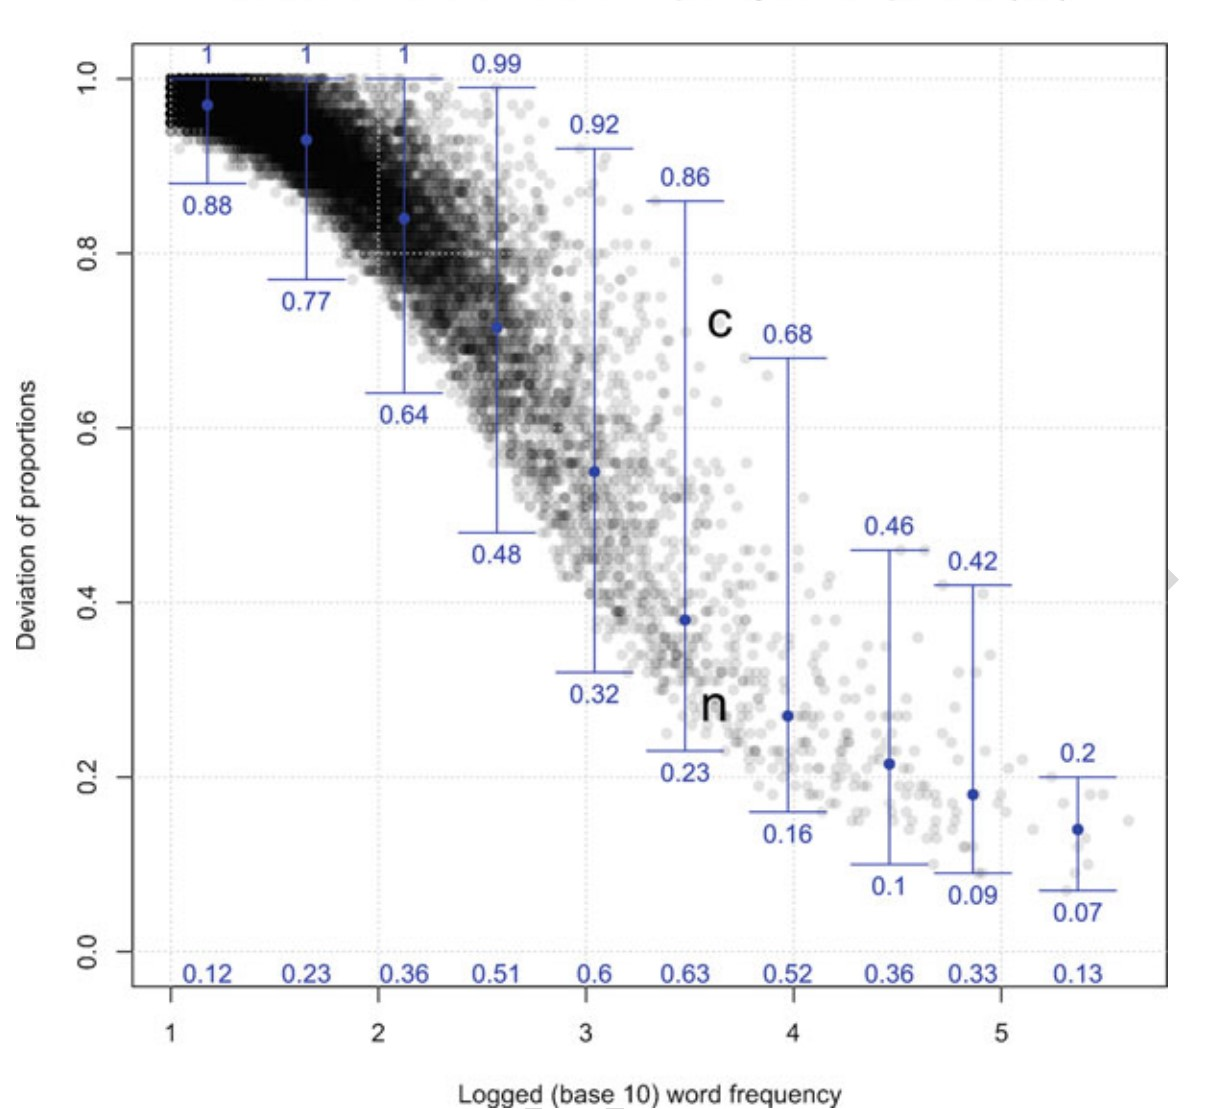
\includegraphics[width=\linewidth]{Gries-frequency-vs-dispersion.jpg}
  \caption[The relation between word frequency and dispersion (DP)]{The relation between word frequency and dispersion ($DP$) \parentext{from \textcite[112]{Gries2021}}}
  \label{fig:Gries-frequency-vs-dispersion}
\end{figure}

Disparities between token frequency and dispersion are especially common for lexical items in the middle frequencies (between $1,000$ and $10,000$ tokens), as demonstrated in \figref{fig:Gries-frequency-vs-dispersion} from \textcite[112]{Gries2021}. In this plot, word frequency is shown on the x-axis (logged to the base of 10), and dispersion is shown on the y-axis (measured using \dfn{Deviation of Proportions} ($DP$); see below for details). Each word in the corpus is represented by a gray point. Lexical items are divided into 10 bins based on frequency, and the blue whisker in each bin represents the range of dispersion values in that frequency bin. The plot makes clear just how widely words within the same frequency bin can vary in terms of their dispersion, especially in the middle frequencies.

If what we are intending to capture with these statistics is some idea of the regularity with which speakers encounter a word, it is clear that raw frequency is a deceptive measure. Instead, recent work has shown that \dfn{corpus dispersion}—how evenly an item is distributed in a corpus—more accurately represents frequency of exposure or lexical access \parencites{Gries2008}{Gries2010}{Griesfc}. Corpus dispersion correlates more strongly with reaction time data than does frequency, for example \parencite{Griesfc}.

Thus for this project I chose to report a measure of corpus dispersion in addition to relative token frequency. Both statistics are provided for the 100-item samples in \appref{app:100-item-samples}. In a review of various measures of corpus dispersion, \textcite{Gries2008} discusses shortcomings with existing measures and proposes a conceptually simple alternative measure, \dfn{Deviation of Proportions} ($DP$) (it is also this measure which most strongly correlates with reaction time data, as mentioned above). In essence, Deviation of Proportions measures how much the frequency of an item within the various parts of a corpus deviates from what one would expect if the item were evenly distributed in the corpus. The procedure for calculating $DP$ for a given lexical item is as follows:

\begin{enumerate}
  \item Determine the sizes of each part of the corpus as a percentage of the overall corpus. These values represent the \emph{expected} percentage of the time that one would expect the item to appear in each corpus part, if it were evenly distributed.
  \item Determine the frequencies with with the target item occurs in each part, as a percentage of its overall frequency of occurrence. These values represent the \emph{actual} or \emph{observed} percentage of the time that the item apperas in each corpus part.
  \item Compute the pairwise absolute differences between the expected and observed percentages, sum them up, and divide the result by two.
  \item The result is $DP$, which theoretically ranges from $0$ (the item is evenly distributed across the corpus, given the size of the parts) to $1$ (the item is unevenly distributed across the corpus, given the size of the parts).
\end{enumerate}

\noindent The mathematical formulization of $DP$ is shown in \exref{ex:DP}, where $n$ is the number of corpus parts, $v$ is the frequencies of the target item in each corpus part, $f$ is the overall frequency of the target item in the corpus, and $s$ is the percent size of each corpus part.

\begin{exe}
  \ex\label{ex:DP}
  $DP = 0.5 \times \displaystyle\sum_{i = 1}^{n}|\frac{v_i}{f} - s_i|$
\end{exe}

\noindent A more detailed explanation of this calculation, with examples, is in \textcite[§3]{Gries2008}. Note that while the theoretical range of $DP$ is between $0$ and $1$, it will never actually reach these two limits because a particular proportion of the lexical item was expected to occur in each corpus part anyway. This issue is only noticeable in corpora with a very small number of parts.

\section{Summary}
\label{sec:3.5}

This chapter has presented the methodological tools necessary for answering the research questions put forth in \chref{ch:introduction}. The methods adopted in this study are novel for several reasons. First, this is the first study to utilize naturalistic discourse data from corpora to examine lexical flexibility at the level of the individual lexical item. Second, this is the first study to \emph{quantify} the lexical flexibility of individual lexical items, in a crosslinguistically applicable way. The calculation of lexical flexibility using Shannon's $H$ is intended as the main methodological contribution of this thesis. Finally, this study incorporates findings from recent research in corpus linguistics which suggest that corpus dispersion is a better measure of frequency of exposure than just raw token frequency. As such, I report on both token frequency and corpus dispersion and examine their interaction as they relate to lexical flexibility in \addcrossref{Section XX}. With these methodological prerequisites in place, I now turn to answering this study's research questions in \chref{ch:results}.
